\subsection*{Problèmes évolutifs}
\textbf{Méthode explicite:}
\begin{equation*}
    \boxed{\frac{\mathrm{d}\overrightarrow{u_h}(t_k)}{\mathrm{d}t}\approx \frac{\overrightarrow{u_h}(t_k+\tau)-\overrightarrow{u_h}(t_k)}{\tau}=\frac{\overrightarrow{u_h}^{(k+1)}-\overrightarrow{u_h}^{(k)}}{\tau}}
\end{equation*}
Puis faire Euler, Heun, Runge-Kutta (voir formulaire CompAlg).
Il faut que $\tau$ soit suffisamment petit pour que la méthode soit stable:
\begin{equation*}
    \tau\leq \frac{2}{\lambda_{max}}
\end{equation*}
$\lambda_{max}$ est la plus grande valeur propre de la matrice $A$ du problème de Cauchy.\\
\textbf{Méthode implicite:}
\begin{equation*}
    \boxed{\frac{\mathrm{d}\overrightarrow{u_h}(t_{k+1})}{\mathrm{d}t}\approx \frac{\overrightarrow{u_h}(t_{k+1})-\overrightarrow{u_h}(t_{k+1}-\tau)}{\tau}=\frac{\overrightarrow{u_h}^{(k+1)}-\overrightarrow{u_h}^{(k)}}{\tau}}
\end{equation*}
\textbf{Exemple:}\\
Soit le problème suivant:
\begin{figure}[H]
    \centering
    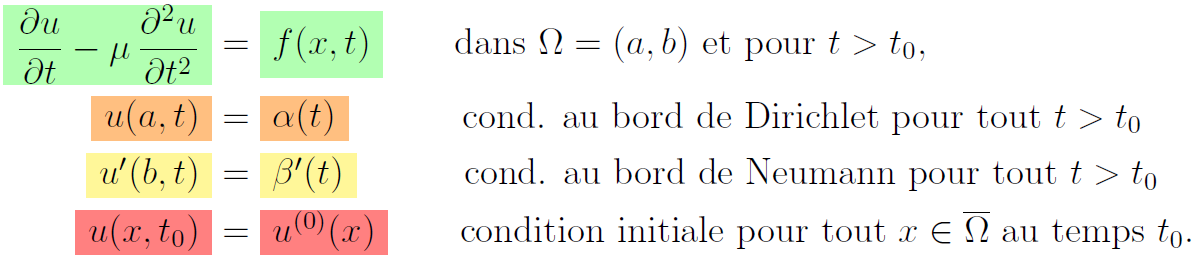
\includegraphics[width=\columnwidth]{images/semaine12_exemple_evolutif1.png}
\end{figure}
\underline{Semi-discrétisation en espace:}\\
Discrétiser l'équation par les différences finies centrées en espace et préparer le
problème de Cauchy pour l'itération en temps:
\begin{figure}[H]
    \centering
    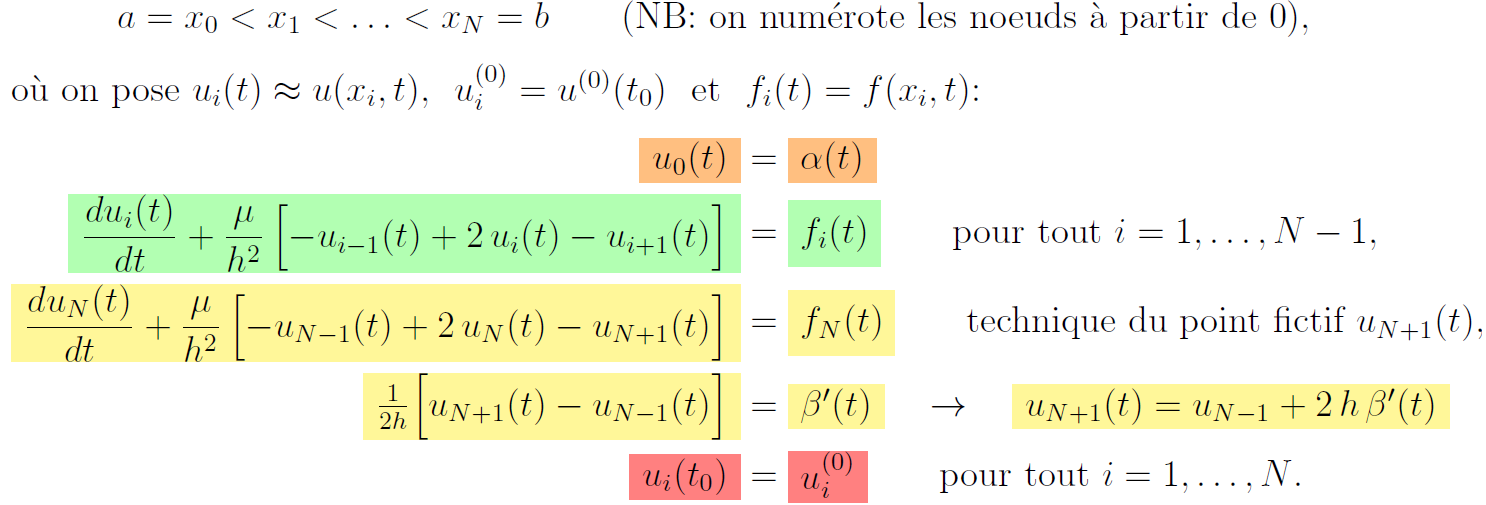
\includegraphics[width=\columnwidth]{images/semaine12_exemple_evolutif2.png}
\end{figure}
Eliminer la valeur fictive $u_{N+1}(t)$ et la valeur de la condition au bord
$u_0(t)=\alpha(t)$:
\begin{figure}[H]
    \centering
    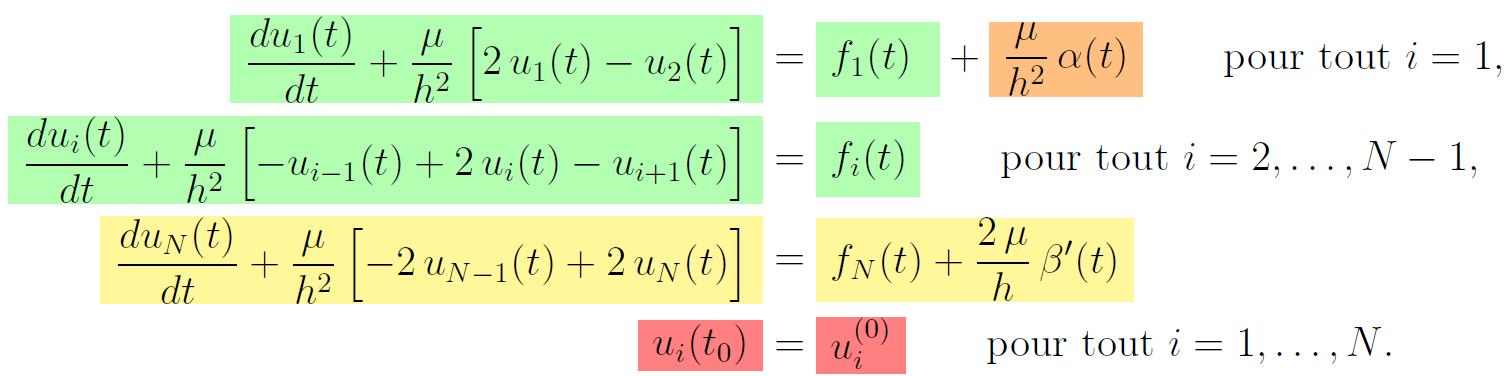
\includegraphics[width=\columnwidth]{images/semaine12_exemple_evolutif3.png}
\end{figure}
Sous forme matricielle:
\begin{figure}[H]
    \centering
    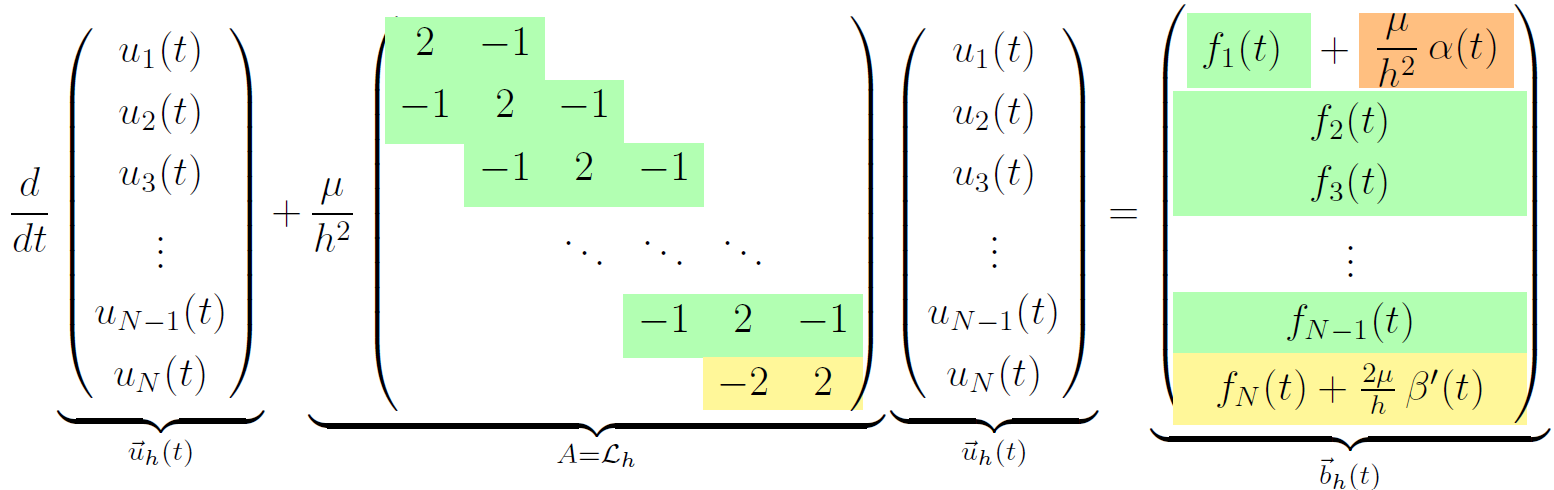
\includegraphics[width=\columnwidth]{images/semaine12_exemple_evolutif4.png}
\end{figure}
\begin{figure}[H]
    \centering
    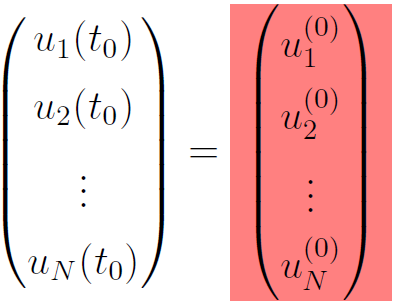
\includegraphics[width=0.3\columnwidth]{images/semaine12_exemple_evolutif5.png}
\end{figure}
Pour obtenir le \underline{problème de Cauchy}, on isole $\frac{\mathrm{d}\overrightarrow{u_h}(t)}{\mathrm{d}t}$
\begin{equation*}
    \boxed{\frac{\mathrm{d}\overrightarrow{u_h}(t)}{\mathrm{d}t}=\underbrace{\overrightarrow{b_h}(t)-A\overrightarrow{u_h}(t)}_{\overrightarrow{f}(t,\overrightarrow{u_h}(t))}}
\end{equation*}
\underline{Discrétisation:}\\
connaisant la solution exacte $u(x,t)$:
\begin{equation*}
    u(x,t)=e^{-\mu t}x\cos(x)+e^{-\frac{4}{9}\pi^2\mu t}\sin(\frac{3\pi}{2}x)
\end{equation*}
On peut calculer $u_i(0)$:
\begin{equation*}
    u_i(0)=u(x_i,0)=x_i\cos(x_i)+\sin(\frac{3\pi}{2}x_i)
\end{equation*}
\underline{Résolution numérique:}\\
Avec Euler, Heun, Runge-Kutta on itère en temps, dans ce cas on prend Euler:
\begin{equation*}
    \overrightarrow{u_h}^{(0)}=
    \begin{pmatrix}
        x_1\cos(x_1)+\sin(\frac{3\pi}{2}x_1) \\
        x_2\cos(x_2)+\sin(\frac{3\pi}{2}x_2) \\
        \vdots                               \\
        x_N\cos(x_N)+\sin(\frac{3\pi}{2}x_N) \\
    \end{pmatrix}
\end{equation*}

